\documentclass[11pt]{article}
\usepackage[margin=1in]{geometry}
\usepackage{amsmath}
\usepackage{amssymb}
\usepackage{enumitem}
\usepackage{xcolor}
\usepackage{tcolorbox}
\usepackage{tikz}
\usetikzlibrary{patterns}

\title{ORF309 Midterm 1 Q2c: Set Subtraction Explained}
\author{}
\date{}

\begin{document}

\maketitle

\section*{What Are We Looking For?}

We want to find:
\[
P(S_P \in [1,2), \, S_N \in [1,2))
\]

This means: \textbf{Princeton gets between 1 and 2 feet (not including 2) AND New York gets between 1 and 2 feet (not including 2)}.

\section*{The Notation}

Define $A_{xy} = \{S_P \geq x, S_N \geq y\}$, which means ``Princeton gets at least $x$ feet AND New York gets at least $y$ feet.''

So:
\begin{align*}
A_{11} &= \{S_P \geq 1, S_N \geq 1\} \quad \text{(both get at least 1 foot)} \\
A_{12} &= \{S_P \geq 1, S_N \geq 2\} \quad \text{(Princeton $\geq$ 1 foot, NY $\geq$ 2 feet)} \\
A_{21} &= \{S_P \geq 2, S_N \geq 1\} \quad \text{(Princeton $\geq$ 2 feet, NY $\geq$ 1 foot)} \\
A_{22} &= \{S_P \geq 2, S_N \geq 2\} \quad \text{(both get at least 2 feet)}
\end{align*}

From the problem, we know:
\begin{align*}
P(A_{11}) &= \frac{1}{3} \\
P(A_{12}) &= \frac{1}{4} \\
P(A_{21}) &= \frac{1}{4} \\
P(A_{22}) &= \frac{1}{5}
\end{align*}

\section*{The Key Insight: Set Subtraction}

Let $A^* = \{S_P \in [1,2), S_N \in [1,2)\}$ be the event we want.

\subsection*{Breaking Down $A^*$}

$S_P \in [1,2)$ means $1 \leq S_P < 2$, which is the same as:
\[
(S_P \geq 1) \text{ AND } (S_P < 2)
\]

Similarly for $S_N \in [1,2)$.

So $A^*$ means:
\begin{itemize}
    \item Both get \textbf{at least 1 foot} (i.e., we're in $A_{11}$)
    \item \textbf{BUT} Princeton does NOT get 2 or more feet
    \item \textbf{AND} New York does NOT get 2 or more feet
\end{itemize}

\subsection*{Visualizing the Problem}

Think of $A_{11}$ as the big region where both get at least 1 foot.

Inside $A_{11}$, we need to \textbf{remove} cases where:
\begin{itemize}
    \item Princeton gets $\geq$ 2 feet (while NY gets $\geq$ 1 foot) — this is $A_{21}$
    \item New York gets $\geq$ 2 feet (while Princeton gets $\geq$ 1 foot) — this is $A_{12}$
\end{itemize}

\begin{tcolorbox}[colback=blue!10, colframe=blue!50!black, title=The Formula]
\[
A^* = A_{11} \setminus (A_{12} \cup A_{21})
\]

In words: ``Both get at least 1 foot'' MINUS ``at least one of them gets 2 or more feet.''
\end{tcolorbox}

\section*{Computing $P(A^*)$}

Using the set subtraction formula:
\[
P(A^*) = P(A_{11}) - P(A_{12} \cup A_{21})
\]

\subsection*{Step 1: Find $P(A_{12} \cup A_{21})$}

Using the inclusion-exclusion principle:
\[
P(A_{12} \cup A_{21}) = P(A_{12}) + P(A_{21}) - P(A_{12} \cap A_{21})
\]

\subsection*{Step 2: Find $P(A_{12} \cap A_{21})$}

$A_{12} \cap A_{21}$ means:
\begin{itemize}
    \item From $A_{12}$: $S_P \geq 1$ and $S_N \geq 2$
    \item From $A_{21}$: $S_P \geq 2$ and $S_N \geq 1$
\end{itemize}

Taking the intersection (both must be true):
\[
A_{12} \cap A_{21} = \{S_P \geq 2, S_N \geq 2\} = A_{22}
\]

So:
\[
P(A_{12} \cap A_{21}) = P(A_{22}) = \frac{1}{5}
\]

\subsection*{Step 3: Plug In}

\begin{align*}
P(A_{12} \cup A_{21}) &= P(A_{12}) + P(A_{21}) - P(A_{22}) \\
&= \frac{1}{4} + \frac{1}{4} - \frac{1}{5} \\
&= \frac{5}{20} + \frac{5}{20} - \frac{4}{20} \\
&= \frac{6}{20} = \frac{3}{10}
\end{align*}

\subsection*{Step 4: Final Answer}

\begin{align*}
P(A^*) &= P(A_{11}) - P(A_{12} \cup A_{21}) \\
&= \frac{1}{3} - \frac{3}{10} \\
&= \frac{10}{30} - \frac{9}{30} \\
&= \frac{1}{30} \\
&\approx 0.033
\end{align*}

\section*{Why This Approach Works}

\begin{enumerate}
    \item We start with $A_{11}$: all cases where both get at least 1 foot.

    \item We subtract $A_{12} \cup A_{21}$: all cases where at least one of them gets 2 or more feet.

    \item What's left is exactly the cases where \textbf{both are in [1, 2)}.
\end{enumerate}

\section*{Common Mistake}

\begin{tcolorbox}[colback=red!10, colframe=red!50!black, title=Wrong Approach]
\textbf{WRONG:}
\[
P(A^*) \neq P(A_{11}) - P(A_{22})
\]

This would miss the cases where:
\begin{itemize}
    \item Princeton gets $\geq 2$ feet but NY is in [1, 2)
    \item NY gets $\geq 2$ feet but Princeton is in [1, 2)
\end{itemize}
\end{tcolorbox}

\section*{Visual Intuition}

Think of it like this:

\begin{center}
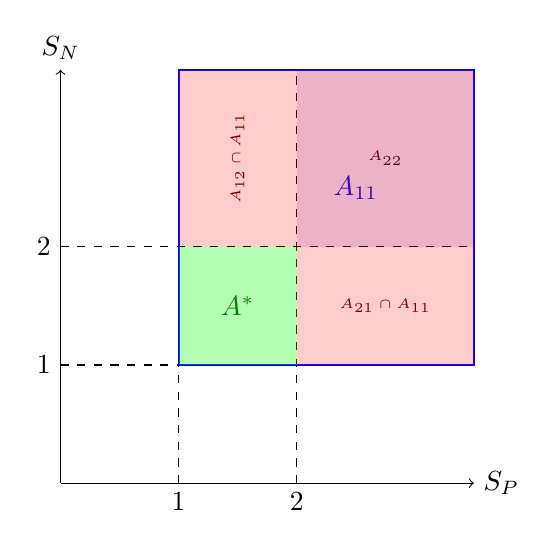
\begin{tikzpicture}[scale=1.5]
    % Draw axes
    \draw[->] (0,0) -- (3.5,0) node[right] {$S_P$};
    \draw[->] (0,0) -- (0,3.5) node[above] {$S_N$};

    % Mark key points
    \draw[dashed] (1,0) -- (1,3.5);
    \draw[dashed] (2,0) -- (2,3.5);
    \draw[dashed] (0,1) -- (3.5,1);
    \draw[dashed] (0,2) -- (3.5,2);

    % Labels
    \node[below] at (1,0) {1};
    \node[below] at (2,0) {2};
    \node[left] at (0,1) {1};
    \node[left] at (0,2) {2};

    % A_11 region (large square)
    \draw[thick, blue] (1,1) rectangle (3.5,3.5);
    \node[blue] at (2.5,2.5) {$A_{11}$};

    % A* region (what we want)
    \fill[green, opacity=0.3] (1,1) rectangle (2,2);
    \node[green!50!black, font=\bfseries] at (1.5,1.5) {$A^*$};

    % A_21 region (right strip)
    \fill[red, opacity=0.2] (2,1) rectangle (3.5,2);
    \node[red!50!black] at (2.75,1.5) {\tiny $A_{21} \cap A_{11}$};

    % A_12 region (top strip)
    \fill[red, opacity=0.2] (1,2) rectangle (2,3.5);
    \node[red!50!black, rotate=90] at (1.5,2.75) {\tiny $A_{12} \cap A_{11}$};

    % A_22 region (top-right corner)
    \fill[purple, opacity=0.3] (2,2) rectangle (3.5,3.5);
    \node[purple!50!black] at (2.75,2.75) {\tiny $A_{22}$};
\end{tikzpicture}
\end{center}

\begin{itemize}
    \item The big blue square is $A_{11}$ (both $\geq 1$)
    \item The small green square is $A^*$ (both in [1,2))
    \item The red regions are where at least one is $\geq 2$ (we subtract these)
    \item The purple corner is $A_{22}$ (both $\geq 2$)
\end{itemize}

\section*{Summary}

To find $P(S_P \in [1,2), S_N \in [1,2))$:

\begin{enumerate}
    \item Start with $P(A_{11}) = \frac{1}{3}$ (both $\geq 1$)
    \item Subtract $P(A_{12} \cup A_{21})$ (at least one $\geq 2$)
    \item Use inclusion-exclusion: $P(A_{12} \cup A_{21}) = \frac{1}{4} + \frac{1}{4} - \frac{1}{5} = \frac{3}{10}$
    \item Final answer: $\frac{1}{3} - \frac{3}{10} = \frac{1}{30}$
\end{enumerate}

\end{document}
